\documentclass{article}

\usepackage{geometry}
\usepackage{graphicx}
\usepackage{physics}


\title{Exercise 1, TFY4235 Computational physics}
\author{Martin K. Johnsrud}
\vspace{-8ex}
\date{}

\begin{document}
    \maketitle
    \section*{Introduction}
        The goal of this exercise is to simulate particles as flat, hard disks in a square, 2D container. This is done with a event-driven simulation, as described in the exercise~\cite{exercise}. This is implemented in Python, using the built-in library heapq. The simulation is used to first tested with scenarios we know the outcome of, then used to demonstrate the Maxwell-Boltzmann distribution and to investigate the effect of a large, heavy disk hitting a large number of small, inert particles.
    
    \section*{Implementation}
        The main engine of the code is the function \verb|run_loop()| in \verb|utillities.py|. It follows the algorithm, as laid out in~\cite{exercise}, using the objects:
        \begin{itemize}
            \item \verb|particles|, a numpy array with the position and velocity of all the particles.
            \item \verb|collisions|, a priority queue containing the time of the collision, the index of the particle(s) involved, and the type of collision it is.
            \item \verb|last_collided|, a list of when each particle was involved in a collision.
        \end{itemize}
        To be expanded \dots

    \section*{Tests}
        Several functions were developed to test the accuracy of the simulation. First, one particle, starting at in the middle of the box, all the way to the left, and with a velocity with at $45^\circ$ to the $x$-axis should move in a titled rectangle. With $\xi=1$ it should also conserve energy. Figure \ref{single particle} shows that this is still the case after $10,000$ events. To test the validity of the particle collision, one small, light particle is sent towards a single, large and heavy particle, with varying impact parameters. The relationship between the impact parameter is is (ref til goldstein, begunn hvorfor det blir cos) $\dv{s}{\theta} = a / 2 \sin(\theta / 2)$. The result is shown i Figure \ref{scattering}, and is in good agreement with the theory. Lastly, the energy from a simulation of $N$ particles over $T$ events is shown in

        \begin{figure}
            \centering
            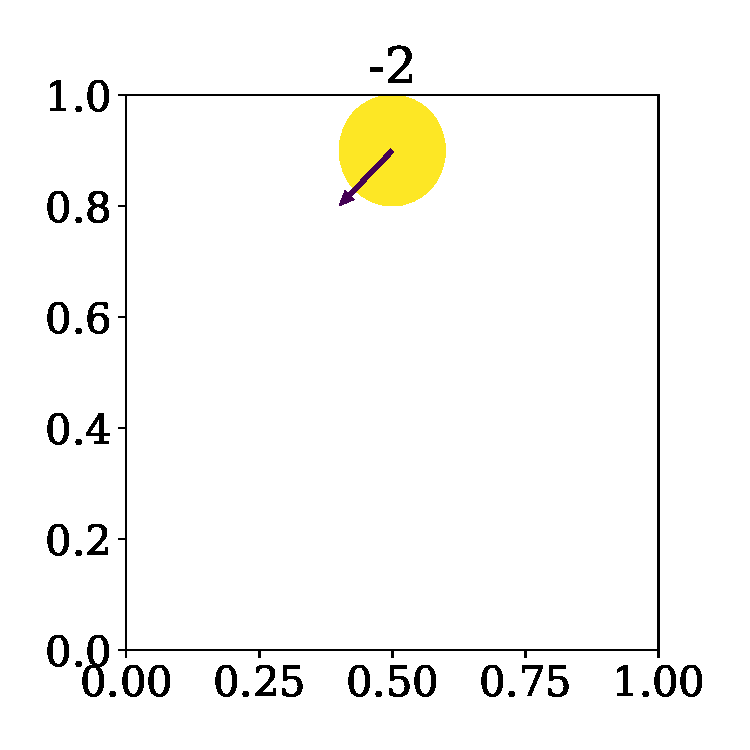
\includegraphics[width=0.49\textwidth]{../plots/test_case_one_particle/particle-2.pdf}
            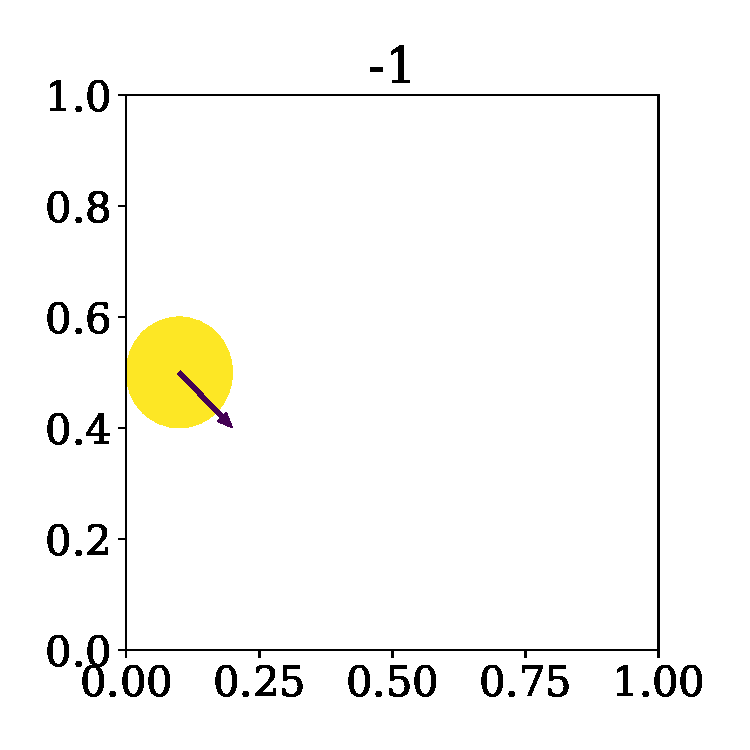
\includegraphics[width=0.49\textwidth]{../plots/test_case_one_particle/particle-1.pdf}
            \caption{One ball being simulated. after $10 000$ steps, it still follows a regular pattern.}
            \label{single particle}
        \end{figure}

        \begin{figure}
            \centering
            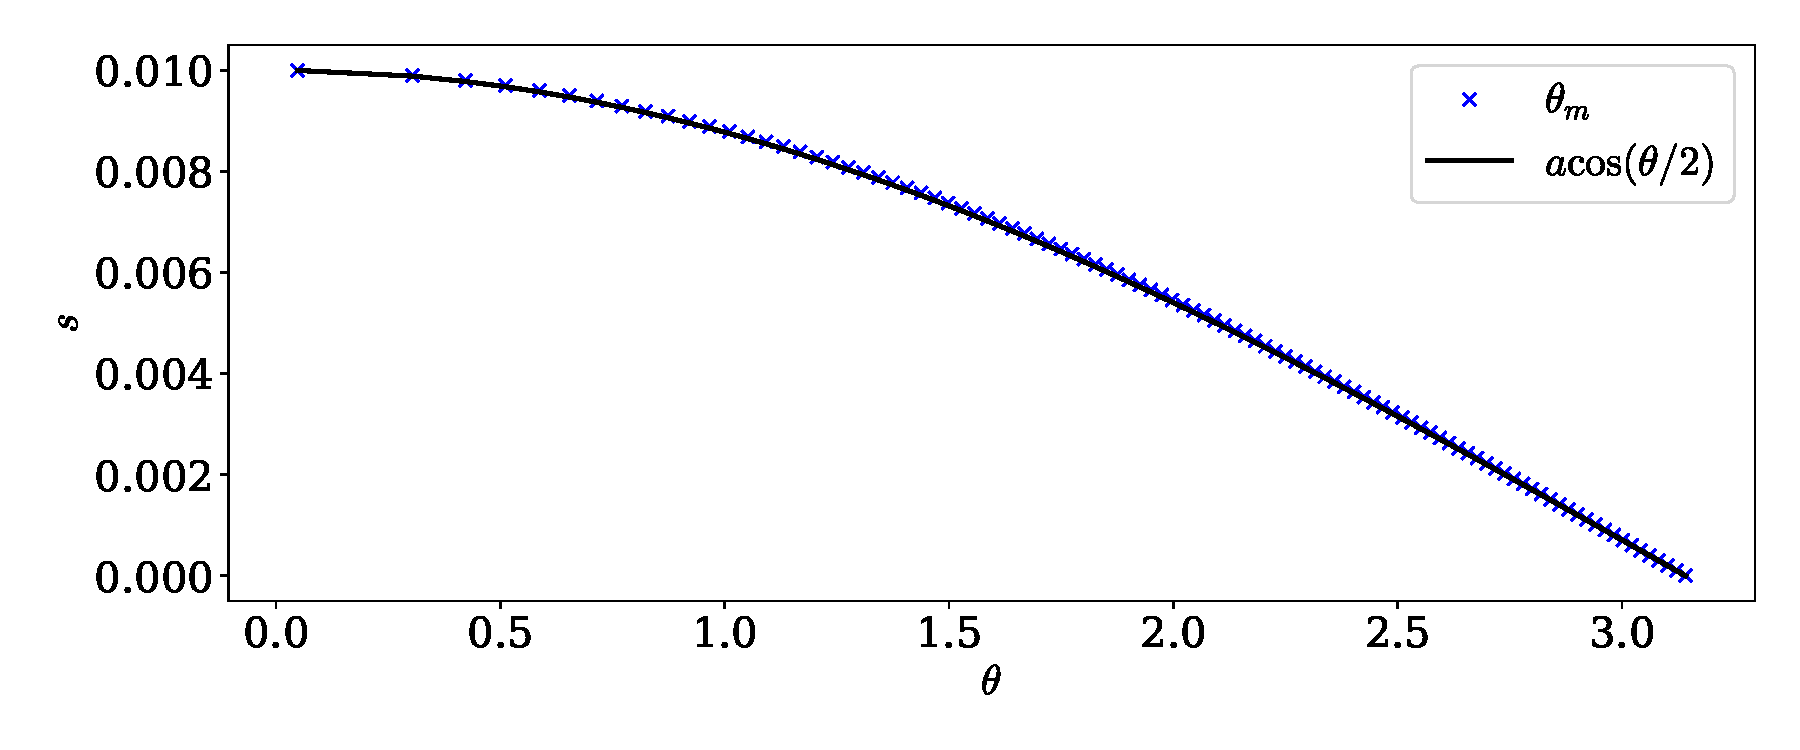
\includegraphics[width=0.8\textwidth]{../plots/test_case_collision_angle/collision_angle.pdf}
            \caption{The }
            \label{scattering}
        \end{figure}

        \begin{figure}
            \centering
            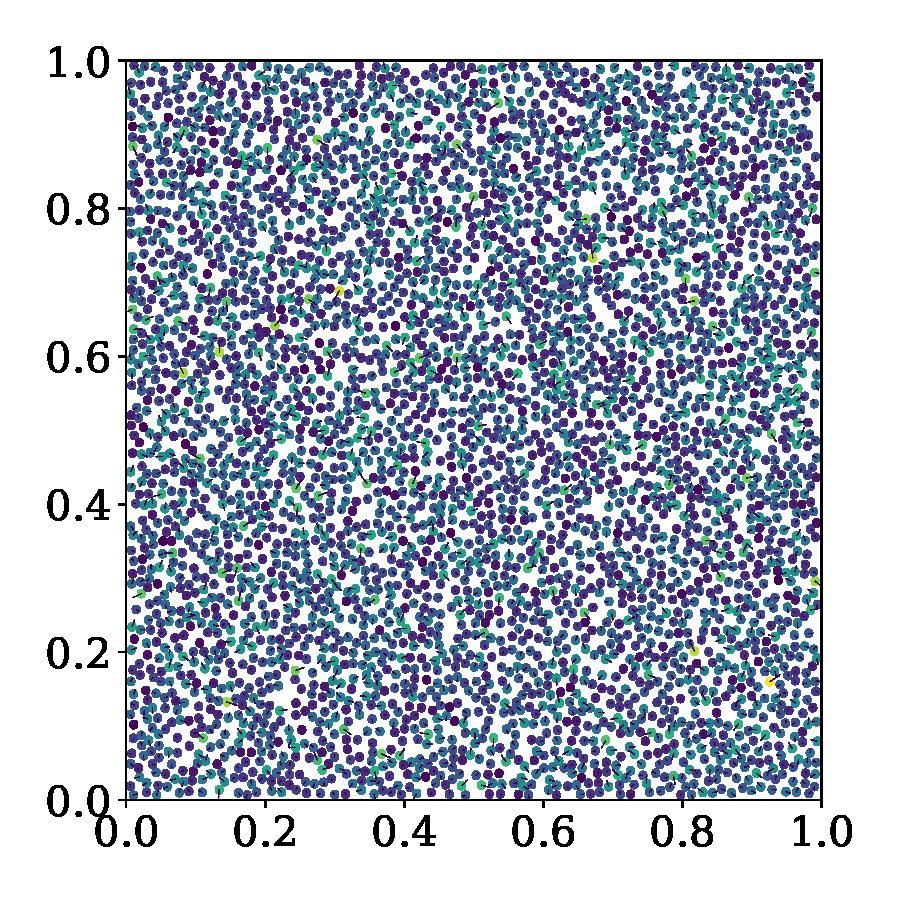
\includegraphics[width=0.49\textwidth]{../plots/test_case_many_particles/test_case_many_particles.pdf}
            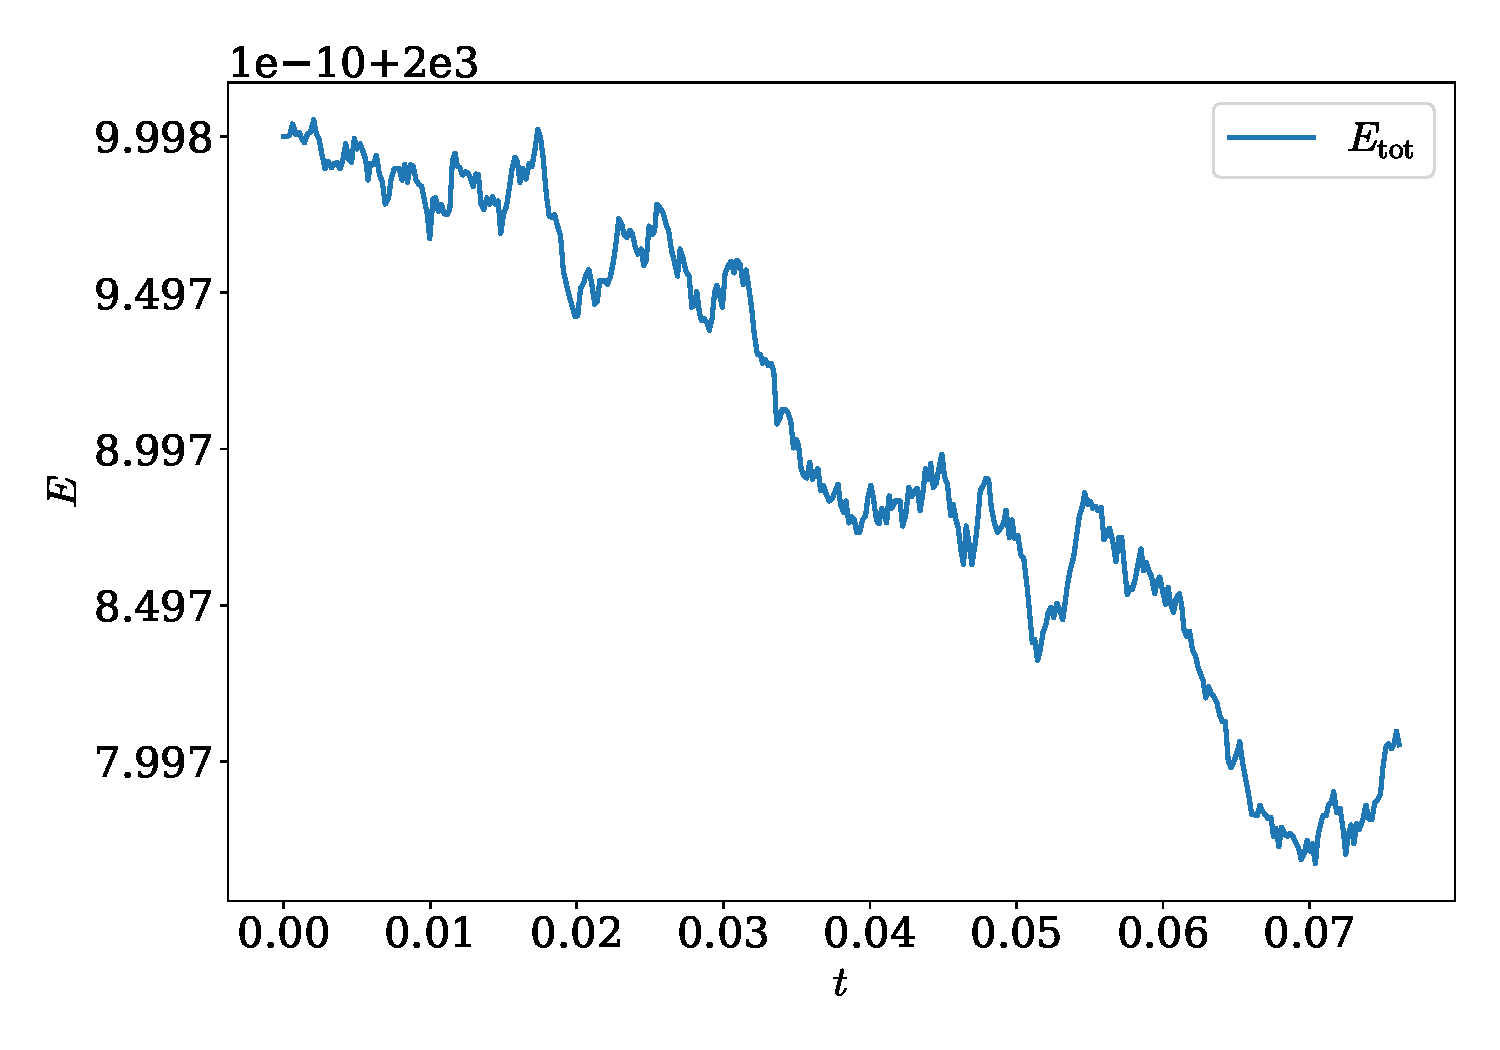
\includegraphics[width=0.49\textwidth]{../plots/test_case_many_particles/energy.pdf}
            \caption{On the left is a snapshot of the particles. The arrows represent the velocities. On the right, the energy is plotted as a function of events. The energy loss can be seen to be negligible.}
        \end{figure}

        \section*{Statistical distribution}
            As the system equilibrates, it should reach the Maxwell-Boltzmann distribution, which in 2D is
            \begin{equation*}
                f(v) = \frac{m v}{T} \exp \left(-\frac{m v^2}{2 T}\right),
            \end{equation*}
            when using units in which $k_b = 1$. The equipartition theorem gives the temperature $T = E$ in 2D. Figure \ref{problem1 av vel} was used to find a good starting point for when the simulation has reach equilibrium. After that, the simulation is sampled every $N$ event, where $N$ is the number of particles. This ensures somewhat independent samples. Figure \ref{problem1 dist} shows the velocity distribution, compared to the Maxwell Boltzmann distribution

            \begin{figure}
                \centering
                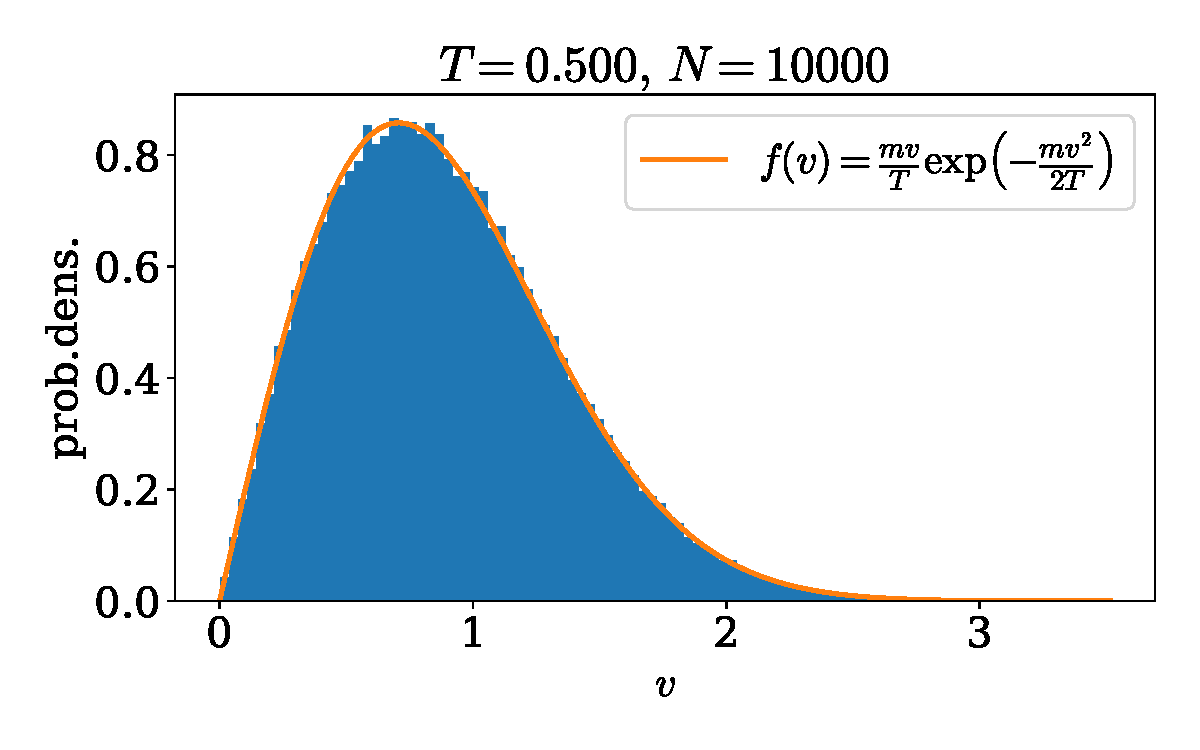
\includegraphics[width=0.8\textwidth]{../plots/problem1/vel_dist.pdf}
                \caption{The velocity distribution is a good fit with the Maxwell-Boltzmann distribution, shown as a blue line.}
                \label{problem1 dist}
            \end{figure}
            \begin{figure}
                \centering
                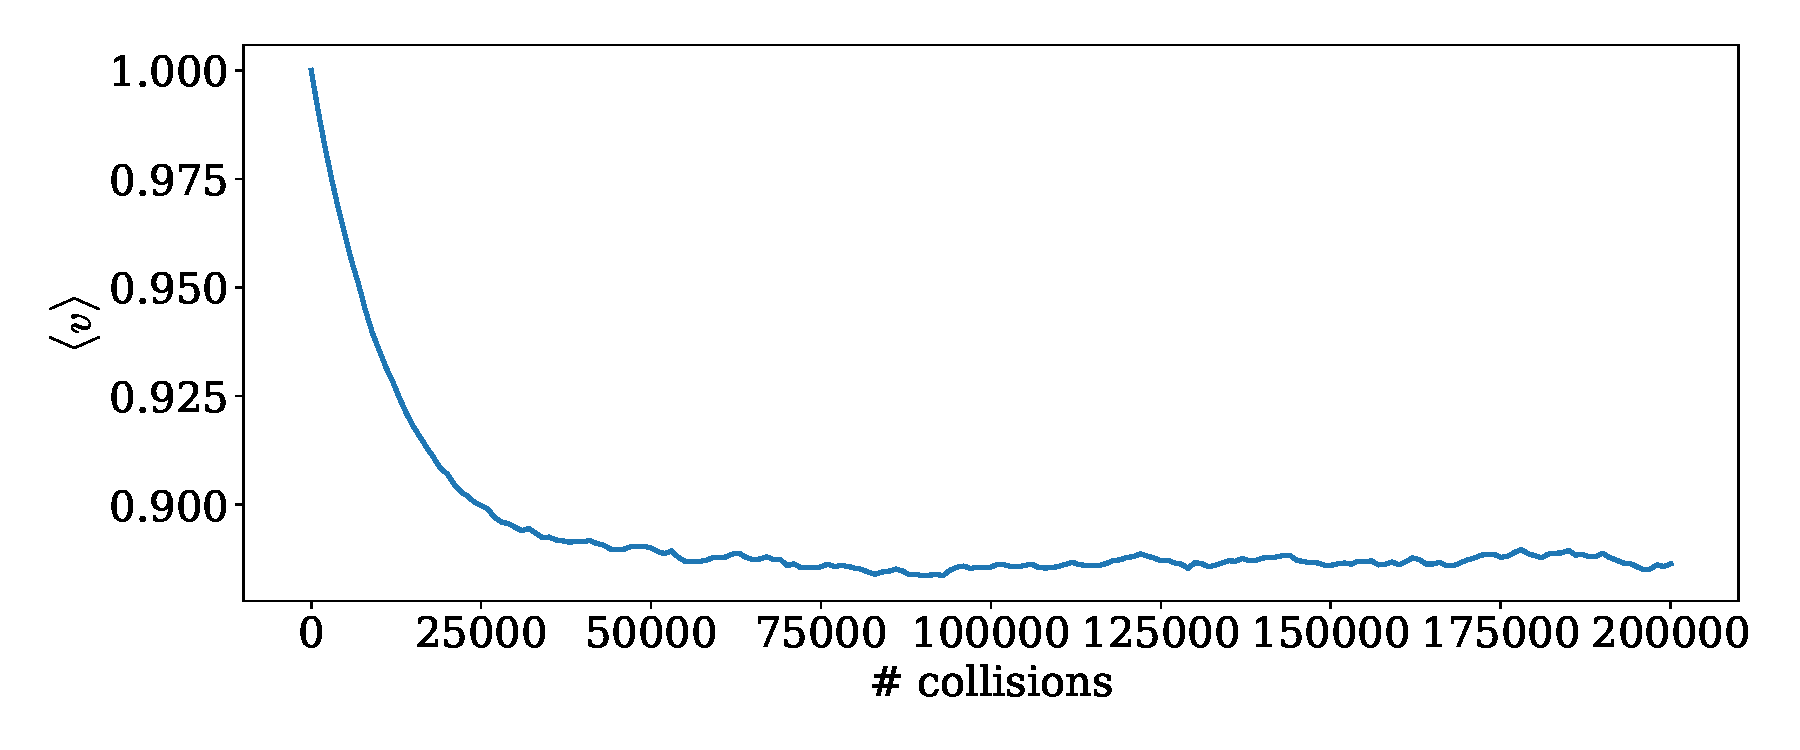
\includegraphics[width=0.8\textwidth]{../plots/problem1/v_av.pdf}
                \caption{Average velocity, as a function of collisions. The distribution reaches equilibrium around $6000$ collisions, or $3N$}
                \label{problem1 av vel}
            \end{figure}
    

    \bibliography{report}
    \bibliographystyle{plain}   
\end{document}